\chapter{The Economic Problem (Text Ch. 2)}

\section{Production possibilities and opportunity cost}

\begin{definition}[Production possibilities frontier]
The \emph{production possibilities frontier} (PPF) is the boundary between the
combinations of goods and services that can be produced and those that cannot. It shows
the maximum combinations of outputs that can be produced with the given resources and
technology, holding the quantities of all other goods constant.
\end{definition}

\begin{example}[A PPF for pizza and cola]
An economy that produces only pizza (millions per year) and cola (millions of cans per
year) has the following production possibilities:
\begin{center}
\begin{tabular}{cccc}
\toprule
Possibility & Pizza & Cola & Opportunity cost of one more pizza \\
\midrule
A & 0 & 15 & -- \\
B & 1 & 14 & 1 can \\
C & 2 & 12 & 2 cans \\
D & 3 & 9 & 3 cans \\
E & 4 & 5 & 4 cans \\
F & 5 & 0 & 5 cans \\
\bottomrule
\end{tabular}
\end{center}
Moving from C to D gains 1 pizza and gives up $12 - 9 = 3$ cans, so the opportunity
cost of the third pizza is 3 cans of cola.
\end{example}

\begin{center}
\begin{tikzpicture}[xscale=1.1, yscale=0.33]
  \draw[->] (0,0) -- (7,0) node[right] {Pizza};
  \draw[->] (0,0) -- (0,17) node[above] {Cola};
  \draw[thick, blue] plot[smooth] coordinates {(0,15) (1,14) (2,12) (3,9) (4,5) (5,0)};
  \foreach \x/\y/\n in {0/15/A, 1/14/B, 2/12/C, 3/9/D, 4/5/E, 5/0/F}
    \node[circle, fill, inner sep=1.3pt, label=above right:{\n}] at (\x,\y) {};
  \node[circle, fill=red, inner sep=1.3pt, label={[red]below left:Z (inefficient)}] at (1.5,6) {};
  \node[circle, fill=red, inner sep=1.3pt, label={[red]above right:W (unattainable)}] at (4,11) {};
  \node[blue] at (5.6,4) {PPF};
\end{tikzpicture}
\end{center}

\subsection{Production efficiency}

\begin{definition}[Production efficiency]
\emph{Production efficiency} is achieved when we cannot produce more of one good without
producing less of some other good. Every point \emph{on} the PPF is production efficient.
\end{definition}

Points \emph{inside} the PPF (like Z) are attainable but inefficient: resources are
unemployed or misallocated (e.g.\ in a recession). Points \emph{outside} (like W) are
unattainable with current resources and technology.

\subsection{Trade-offs and opportunity cost along the PPF}

Every choice along the PPF involves a trade-off: to get more of one good we must give up
some of the other. The opportunity cost is a \emph{ratio}:
\[
  \text{opportunity cost of a pizza}
  = \frac{\text{decrease in cola}}{\text{increase in pizza}},
\]
and the opportunity cost of cola is the inverse of the opportunity cost of pizza. Between
D and E the opportunity cost of a pizza is 4 cans, so the opportunity cost of a can is
$1/4$ pizza.

\subsection{Increasing opportunity cost}

As production of pizza increases, the opportunity cost of each extra pizza rises
(1, 2, 3, 4, 5 cans above). This is why the PPF \emph{bows outward} (is concave to the
origin). The reason is that resources are not equally productive in all activities:
the first resources moved into pizza are the ones best suited to pizza and worst suited to
cola; later we must move resources that are very good at making cola.

\begin{important}[Pitfall]
A straight-line PPF means \emph{constant} opportunity cost (resources equally productive
in both uses). A bowed-out PPF means \emph{increasing} opportunity cost. Do not confuse
the slope of the PPF with the quantity produced.
\end{important}

\section{Using resources efficiently}

Production efficiency picks out the points on the PPF, but which point is best? That
requires comparing costs and benefits at the margin.

\subsection{Marginal cost}

\begin{definition}[Marginal cost]
The \emph{marginal cost} of a good is the opportunity cost of producing one more unit of
it. Marginal cost increases as more is produced, which is the increasing opportunity
cost read off the PPF. The marginal cost curve slopes upward.
\end{definition}

\subsection{Preferences and marginal benefit}

\begin{definition}[Marginal benefit]
The \emph{marginal benefit} of a good or service is the benefit received from consuming
one more unit of it. It is measured by the most that people are willing to pay (in money
or in other goods) for an additional unit.
\end{definition}

\begin{important}[Principle of decreasing marginal benefit]
The more we have of any good or service, the smaller is its marginal benefit and the less
we are willing to pay for an additional unit. The marginal benefit curve slopes downward.
\end{important}

\subsection{Allocative efficiency}

\begin{definition}[Allocative efficiency]
\emph{Allocative efficiency} is achieved when goods and services are produced at the
lowest possible cost and in the quantities that provide the greatest possible benefit.
It occurs at the point on the PPF where marginal benefit equals marginal cost.
\end{definition}

If $MB > MC$ for pizza, society values one more pizza more than what it gives up, so
producing more pizza increases net benefit; if $MB < MC$, produce less. On a graph the
efficient quantity is where the MB and MC curves intersect.

\begin{center}
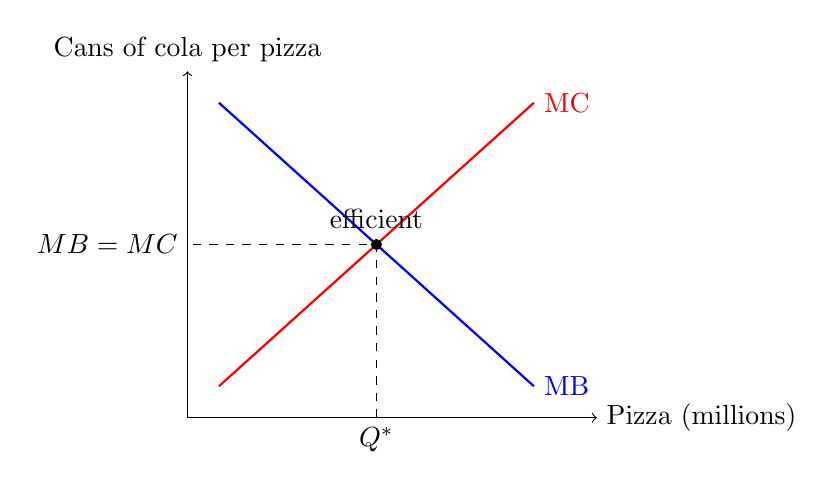
\begin{tikzpicture}[scale=0.8]
  \draw[->] (0,0) -- (6.5,0) node[right] {Pizza (millions)};
  \draw[->] (0,0) -- (0,5.5) node[above] {Cans of cola per pizza};
  \draw[thick, red] (0.5,0.5) -- (5.5,5) node[right] {MC};
  \draw[thick, blue] (0.5,5) -- (5.5,0.5) node[right] {MB};
  \fill (3,2.75) circle (2.5pt);
  \draw[dashed] (3,0) node[below] {$Q^*$} -- (3,2.75) -- (0,2.75) node[left] {$MB=MC$};
  \node[above] at (3,2.85) {efficient};
\end{tikzpicture}
\end{center}

\begin{example}
With the PPF above, suppose people are willing to give up 5 cans for the first pizza, 4
for the second, 3 for the third and 2 for the fourth. Compare with marginal costs of
1, 2, 3, 4 cans. The first two pizzas have $MB > MC$, so producing them adds net
benefit. For the third pizza $MB = MC = 3$ cans, so the efficient output is 3 million
pizzas (point D, with 9 million cans). The fourth pizza costs 4 cans but is worth only 2,
so producing it wastes resources.
\end{example}

\section{Economic growth}

\begin{definition}[Economic growth]
\emph{Economic growth} is the expansion of production possibilities: an outward shift of
the PPF. The two key sources are \emph{technological change} (developing new goods and
better ways of producing them) and \emph{capital accumulation} (growth of capital
resources, including human capital).
\end{definition}

Growth has an opportunity cost: to accumulate capital and develop technology, we must
devote resources to producing capital goods and to research instead of to current
consumption. An economy that chooses more capital goods today (a point higher up on a
``consumption vs capital goods'' PPF) gets a bigger outward shift tomorrow.

\begin{center}
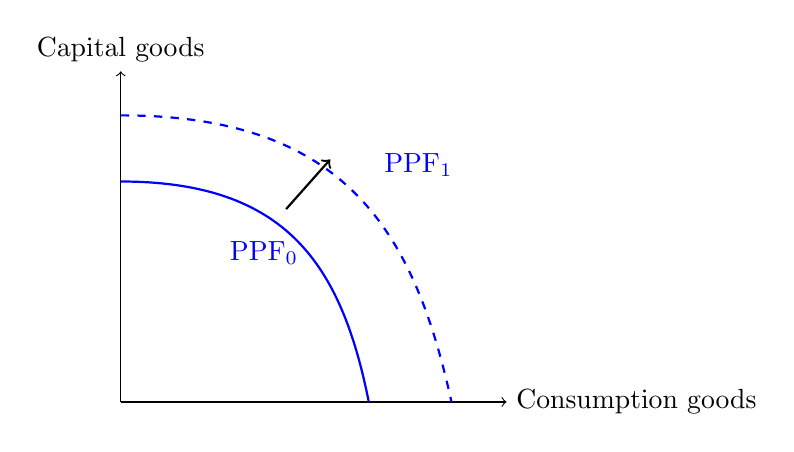
\begin{tikzpicture}[scale=0.7]
  \draw[->] (0,0) -- (7,0) node[right] {Consumption goods};
  \draw[->] (0,0) -- (0,6) node[above] {Capital goods};
  \draw[thick, blue] (0,4) .. controls (3,4) and (4,2.5) .. (4.5,0);
  \draw[thick, blue, dashed] (0,5.2) .. controls (4,5.2) and (5.3,3.2) .. (6,0);
  \node[blue] at (2.6,2.7) {PPF$_0$};
  \node[blue] at (5.4,4.3) {PPF$_1$};
  \draw[->, thick] (3,3.5) -- (3.8,4.4);
\end{tikzpicture}
\end{center}

\begin{remark}
Canada and Hong Kong are classic textbook comparisons: economies that devote a larger
share of resources to capital accumulation grow faster, but they give up current
consumption to do so.
\end{remark}

\section{Gains from trade}

\begin{definition}[Comparative and absolute advantage]
A person (or country) has a \emph{comparative advantage} in an activity if they can
perform it at a \emph{lower opportunity cost} than anyone else. A person has an
\emph{absolute advantage} if they are more productive than others (more output per hour)
in that activity.
\end{definition}

Gains from specialization and trade come from \emph{comparative} advantage, not absolute
advantage. Even someone with an absolute advantage in everything benefits from trading.

\begin{example}[Ann and Bob]
In one day Ann can produce 10 shirts or 20 hats (or any linear combination); Bob can
produce 4 shirts or 16 hats.
\begin{center}
\begin{tabular}{lcc}
\toprule
 & Opportunity cost of 1 shirt & Opportunity cost of 1 hat \\
\midrule
Ann & $20/10 = 2$ hats & $10/20 = 0.5$ shirt \\
Bob & $16/4 = 4$ hats & $4/16 = 0.25$ shirt \\
\bottomrule
\end{tabular}
\end{center}
Ann has an absolute advantage in both goods, but a comparative advantage only in shirts
(2 hats $<$ 4 hats). Bob has a comparative advantage in hats (0.25 shirt $<$ 0.5 shirt).

\emph{No trade}: each spends half the day on each good. Ann makes 5 shirts and 10 hats;
Bob makes 2 shirts and 8 hats. Total: 7 shirts, 18 hats.

\emph{Specialize}: Bob makes only hats (16). Ann spends 0.8 of the day on shirts (8) and
0.2 on hats (4). Total: 8 shirts, 20 hats, more of \emph{both} goods.

\emph{Trade}: Ann gives Bob 3 shirts for 8 hats (a price of $8/3 \approx 2.67$ hats per
shirt, between the two opportunity costs of 2 and 4).
\begin{itemize}
  \item Ann ends with $8-3 = 5$ shirts and $4+8 = 12$ hats (was 5 and 10): gains 2 hats.
  \item Bob ends with 3 shirts and $16-8 = 8$ hats (was 2 and 8): gains 1 shirt.
\end{itemize}
Both consume outside their own PPFs.
\end{example}

\begin{important}[Pitfall]
Trade is mutually beneficial only if the terms of trade lie \emph{between} the two
traders' opportunity costs. Always compare opportunity costs, not output per hour, to find
comparative advantage.
\end{important}

\section{Economic coordination}

Specialization and trade need coordination. Four social institutions make it possible:
\begin{enumerate}
  \item \textbf{Firms}: economic units that hire factors of production and organize them
        to produce and sell goods and services.
  \item \textbf{Markets}: any arrangement that enables buyers and sellers to get
        information and do business with each other. Prices adjust to coordinate
        decisions.
  \item \textbf{Property rights}: the social arrangements that govern ownership, use and
        disposal of resources, goods and services (real, financial and intellectual
        property).
  \item \textbf{Money}: any commodity or token generally acceptable as a means of
        payment; it makes trade far more efficient than barter.
\end{enumerate}

In the \emph{circular flow} model, households sell factors of production to firms in
\emph{factor markets} and receive incomes; firms sell goods and services to households in
\emph{goods markets}; real flows go one way and money flows the other way. This picture
is developed into the GDP accounts in the next chapter.

\section{Summary}

\begin{itemize}
  \item The PPF shows the maximum attainable combinations of output; points on it are
        production efficient, inside is inefficient, outside is unattainable.
  \item Opportunity cost along the PPF is a ratio (decrease in one good over increase in
        the other) and increases because resources are not equally productive everywhere,
        so the PPF bows outward.
  \item Marginal cost rises, marginal benefit falls; allocative efficiency is where
        $MB = MC$.
  \item Growth (technological change, capital accumulation) shifts the PPF outward at the
        cost of current consumption.
  \item Comparative advantage (lowest opportunity cost) drives gains from trade; terms of
        trade must lie between the traders' opportunity costs.
  \item Firms, markets, property rights and money coordinate decisions.
\end{itemize}
